\section{Matched-protocol evidence}
\label{sec:matched}

\paragraph{Original protocol.}
We retrained the production model at reduced depth (six layers, width $48$,
AdamW, sixty epochs, three seeds) in a pre-registered design comparing a
jointly trained linear encoder with encoders frozen at random or PCA
initialization, plus momentum-SGD controls. The joint arm finished
$0.110$ below the frozen-random arm on the pre-specified final-five-epoch
validation macro-F1, a difference that was itself unresolved at three seeds.
The comparison was confounded by three asymmetries: the joint arms trained
the reduction-stage BatchNorm affine parameters, gradient clipping acted on
$\thetap$ and $\phip$ together in joint arms and on $\phip$ alone in frozen
arms, and no best-validation checkpoints were saved. Momentum-SGD controls
showed paired best-validation gaps of $+0.002$ and $+0.011$ and final-five
gaps of $+0.028$ and $-0.057$ at widths $48$ and $192$. Recalibrating
BatchNorm statistics recovers $7$--$17\%$ of the joint arm's peak-to-final
decline for that intervention and those checkpoints.

\paragraph{Matched protocol.}
We reran seven arms at width $48$ with the same clipping rule and scope,
identical treatment of every BatchNorm affine parameter, and saved
best-validation checkpoints (Table~\ref{tab:matched}). The arms form two
matched pairs, not a single-factor design: joint-linear and frozen-random
share a linear reduction with BatchNorm, while frozen-pretrained and
fine-tuned share a pretrained MLP encoder without reduction-stage
BatchNorm, so comparisons across pairs change architecture, training
history and validation selection. The pre-registered predictions were a
fine-tuning deficit relative to the frozen pretrained encoder and a harmful
ordering of spectral learning-rate multipliers.

\begin{table}[t]
\caption{Matched protocol at width $48$, three seeds, mean $\pm$ sd of
validation macro-F1 (best checkpoint, exploratory; final five epochs,
pre-specified) and relative encoder drift $\|\thetap_T-\thetap_0\|/\|\thetap_0\|$.
Validation-selected; no test set; two matched pairs.}
\label{tab:matched}
\begin{center}
\small
\begin{tabular}{lccc}
\toprule
arm & best-val & final-5 & $\thetap$ drift \\
\midrule
frozen random encoder      & $0.814\pm0.040$ & $0.684\pm0.037$ & $0$ \\
joint linear encoder       & $0.837\pm0.029$ & $0.694\pm0.056$ & $0.57$ \\
frozen pretrained encoder  & $0.861\pm0.022$ & $0.690\pm0.033$ & $0$ \\
fine-tuned pretrained      & $0.857\pm0.009$ & $0.710\pm0.052$ & $0.02$ \\
joint, spectral lr $\times0.1$ & $0.841\pm0.007$ & $0.626\pm0.055$ & $0.08$ \\
joint, spectral lr $\times10$  & $0.886\pm0.037$ & $0.561\pm0.114$ & $4.91$ \\
joint, cosine schedule     & $0.825\pm0.033$ & $0.660\pm0.020$ & $0.36$ \\
\bottomrule
\end{tabular}
\end{center}
\end{table}

\paragraph{Verdicts.}
Paired by seed with $90\%$ $t$-intervals ($n=3$), fine-tuning minus the
frozen pretrained encoder is $+0.021$ $[-0.022,+0.063]$ on final-five and
$-0.004$ $[-0.048,+0.039]$ on best-validation: the predicted deficit is not
supported, with verified nonzero applied encoder updates under AdamW.
Joint minus frozen-random is $+0.011$ $[-0.142,+0.163]$ and $+0.023$
$[-0.066,+0.112]$; the original $-0.110$ deficit is absent, and the paired
change in the final-five gap between protocols is $+0.120$
$[-0.230,+0.470]$ (best-validation $-0.010$ $[-0.105,+0.085]$), descriptive
seed summaries only. The $\times10$ multiplier raised best-validation by
$+0.048$ $[-0.016,+0.112]$ in all three seeds while its endpoint fell to
$0.561$ with a fivefold encoder drift; three multiplier means do not
establish a systematic relation between displacement and peak score. This
particular cosine schedule did not improve either mean endpoint. The bound
of Theorem~\ref{thm:twoscale} is not instantiated by these runs, whose
optimizer, clipping and momentum lie outside its hypotheses; a proxy we
computed earlier is withdrawn (Appendix~\ref{app:production}). Disclosures:
one width; three seeds; a single validation fold; no test set;
best-validation is exploratory and final-five pre-specified; pretrained
encoders were selected by macro-F1 on the same validation cores and
pretrained with weight decay $0.01$ on $\thetap$ under an unaugmented
centre-crop protocol, whereas subsequent training used random crops with
augmentation, which affects cross-pair comparisons but not the frozen versus
fine-tuned pair started from the same checkpoint
(Figure~\ref{fig:matched}).

\paragraph{Reading.}
The original protocol confounded freezing with clipping scope and
normalization-parameter treatment. Its nominal final-window freezing
advantage was absent after these differences were removed, while checkpoint
selection reversed the ordering within the original runs. At width $48$ and
three seeds, neither the within-protocol freezing contrasts nor the change
in their gap establishes a population effect. These results demonstrate that
the original contrast cannot identify an architectural shortcut and that
checkpoint policy changes its descriptive conclusion. They support a
protocol-confounded apparent effect; they do not show that architecture has
no effect, nor that the named changes alone caused the earlier difference.

\begin{figure}[t]
\centering
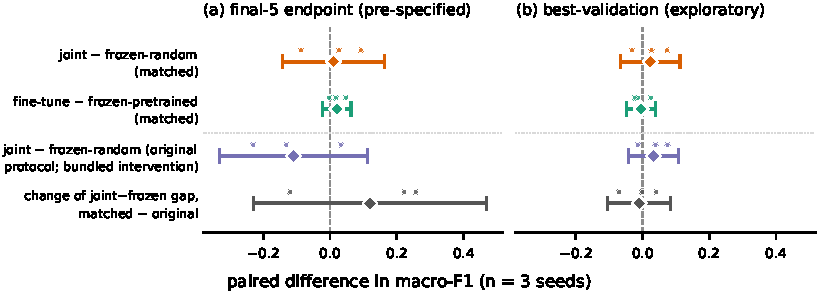
\includegraphics[width=\linewidth]{figures/fig3_matched.pdf}
\caption{Paired arm differences in validation macro-F1 with $90\%$
paired-$t$ intervals ($n=3$; seed points shown). (a) Final five epochs,
pre-specified. (b) Best validation checkpoint, exploratory. The original
joint-minus-frozen contrast is a bundled protocol intervention; the last row
is the change of that gap between protocols.}
\label{fig:matched}
\end{figure}
